\documentclass[14pt]{beamer}

  \usepackage[utf8]{inputenc}
  \usepackage[ngerman]{babel}
  \usepackage{eurosym}
  \usepackage{listings}
  \usepackage{color}

\definecolor{mygreen}{rgb}{0,0.6,0}
\definecolor{mygray}{rgb}{0.5,0.5,0.5}
\definecolor{mymauve}{rgb}{0.58,0,0.82}

\lstset{
 basicstyle=\small,
 backgroundcolor=\color{white},
   numbers=left,
  numbersep=5pt,
  numberstyle=\tiny\color{mygray}, 
  rulecolor=\color{black},  
}
  
  % Hochschule Emden/Leer Layout einbinden
  \usepackage{hs-emden-theme}
  
  % Hochschule Emden/Leer Hintergrundbild einbinden
  \usebackgroundtemplate{
\includegraphics[width=\paperwidth]{logo/hintergrund.eps}}
  
  % Für Grafiken
  \usepackage{float}
  \usepackage{graphicx}
  
  
  % Nummerierung für die Gliederung aktivieren
  \setbeamertemplate{section in toc}[sections numbered]
  
  % Dokumentinformationen
  \author{
    Frederick Lahde
  }
  \title[]{why Docker is not a vm}
  \subtitle{cgroups and namespaces}
  \institute{Hochschule Emden/Leer}
  \date{13.04.2018}
  \subject{Recht und Datenschutz}
  
  \AtBeginSection[]{
    \begin{frame}
      \vfill
      \centering
      \begin{beamercolorbox}[sep=8pt,center,shadow=true,rounded=true]{title}
        \usebeamerfont{title}\insertsectionhead\par%
      \end{beamercolorbox}
      \vfill
    \end{frame}
  }
  
  \begin{document}
    % Titelslide
    \begin{frame}[plain]
      \maketitle
      \centering
      \begin{figure}[H]
        %
\includegraphics[width=0.3\linewidth]{./logo/technik}
      \end{figure}
      \tiny{made with \LaTeX}
    \end{frame}
  
    % Gliederung
    \begin{frame}{Table of contents}
      \setcounter{tocdepth}{1}
      \tableofcontents
    \end{frame}
    
    \section{Docker}
    \begin{frame}{Docker}
    \begin{itemize}
    \item operating-system-level virtualization
    \item dotCloud - 2013, später Adoption von Red Hat
    \item The Docker team, Cisco, Google, Huawei, IBM, Microsoft, Red Hat
    \end{itemize}
    \end{frame}
    
     \begin{frame}{Docker}
    \begin{itemize}
    \item Industriestandart für das Deployment von Applikationen
    \item Konzept von eigenständigen, "statischen" Containern
    \item "Stacks" aus mehren Containern (docker compose)
    \item Orchestrierung von Stacks über Docker Swarm oder Kubernetes
    \item Ist Docker eine VM?
    \end{itemize}
    \end{frame}
    
    \section{cgroups}
    \subsection{Definition}
    \begin{frame}{cgroups - Definition}
    	\begin{itemize}
    	\item control groups
        \item Allokieren von Ressourcen für Gruppen von Prozessen
        \item Monitoring
        \item Umkonfigurieren von cgroups zur Laufzeit
    	\end{itemize}
    \end{frame}
    \subsection{Organisation}
    \begin{frame}{cgroups - Organisation}
    	\begin{itemize}
        \item Mehrere Bäume von cgroups
        \item Jeder Baum hängt an Subsystemen
    	\end{itemize}
    \end{frame}
    \begin{frame}{cgroups - Subsysteme}
    	\begin{itemize}
        \item Repräsentiert eine Ressource
        \item Beispiele in Red Hat:
        	\begin{itemize}
        	\item cpu
            \item devices
            \item freezer
            \item memory
        	\end{itemize}
    	\end{itemize}
    \end{frame}
    
    \subsection{Regeln}
    \begin{frame}{cgroups - Regeln}
    \centering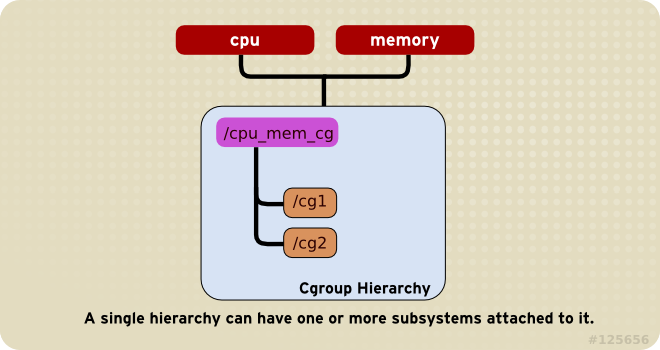
\includegraphics[scale=0.7]{logo/RMG-rule1}
    \end{frame}
    \begin{frame}{cgroups - Regeln}
    \centering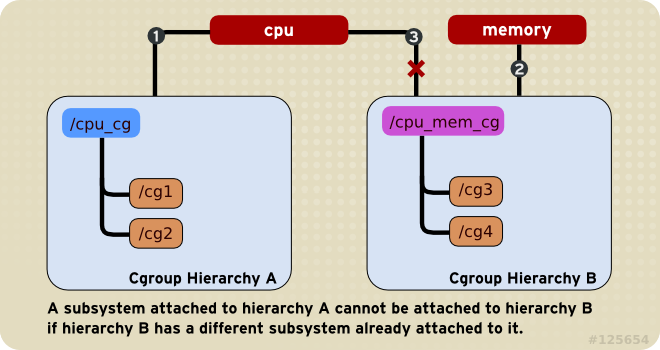
\includegraphics[scale=0.7]{logo/RMG-rule2}
    \end{frame}
    \begin{frame}{cgroups - Regeln}
    \centering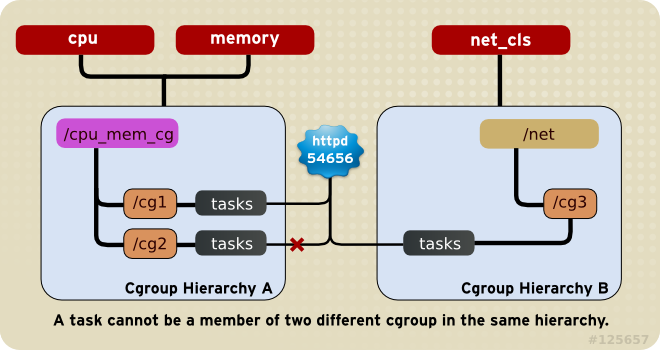
\includegraphics[scale=0.7]{logo/RMG-rule3}
    \end{frame}
    \begin{frame}{cgroups - Regeln}
    \centering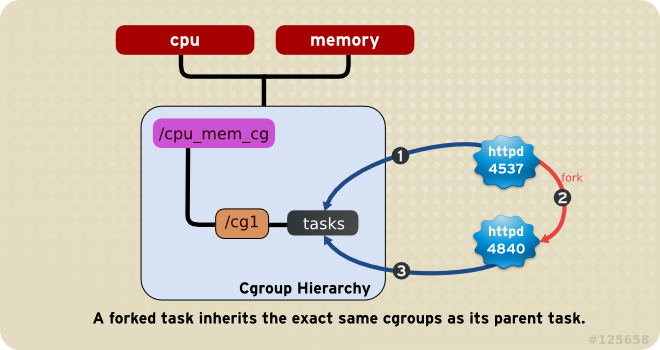
\includegraphics[scale=0.7]{logo/RMG-rule4}
    \end{frame}
    \subsection{Benutzung}
    \begin{frame}{Benutzung}
    \lstinputlisting[title=/etc/cgconfig.conf]{code/cgconfig.conf}
    \end{frame}
    \begin{frame}{Benutzung}
    \lstinputlisting{code/cgroups.sh}
    \end{frame}
    
    \section{namespaces}
    \subsection{Definition}
    \begin{frame}{namespaces - Definition}
    \begin{itemize}
    \item partionieren globale Ressourcen
    \item Sets von Prozessen sehen Sets von Ressourcen
    \item Bestimmmung was ein Prozess vom System sieht
    \end{itemize}
    
    \end{frame}
    \begin{frame}{namespaces - Definition}
    \begin{itemize}
    \item Mount - isolate filesystem mount points
	\item UTS - isolate hostname and domainname
	\item IPC - isolate interprocess communication (IPC) resources
	\item PID - isolate the PID number space
	\item Network - isolate network interfaces
	\item User - isolate UID/GID number spaces
  	\item Cgroup - isolate cgroup root directory
    \end{itemize}
    \end{frame}
    
    \subsection{Benutzung}
    \begin{frame}{Benutzung - Bash}
    \lstinputlisting{code/namespaces-example.sh}
    \end{frame}
    
    \begin{frame}{Benutzung - Golang}
    \lstinputlisting[basicstyle=\tiny]{code/namespaces-example.go}
    \end{frame}
    
    \begin{frame}{Benutzung - Golang}
   	\centering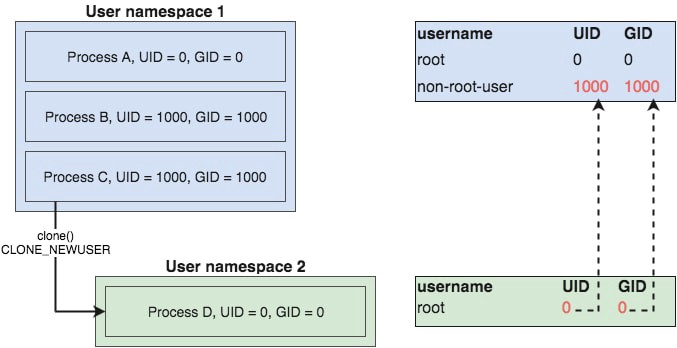
\includegraphics[scale=.4]{logo/user-ns}
    \end{frame}
   
   
    \section{Docker - VM?}
    \subsection{Docker - VM?}
   \begin{frame}{Docker - VM?}
    \begin{itemize}
    \item Basiert auf cgroups und namespaces
    \item Kernel Primitives
    \end{itemize}
    \end{frame}
    
    \begin{frame}{Docker - VM?}
    VMs, Jails, and Zones are if you bought the legos already put together AND glued. So it’s basically the Death Star and you don’t have to do any work you get it pre-assembled out of the box. You can’t even take it apart.
    \tiny Jessie Frazelle
	\end{frame}
    \begin{frame}{Docker - VM?}
Containers come with just the pieces so while the box says to build the Death Star, you are not tied to that. You can build two boats connected by a flipping ocean and no one is going to stop you.
	\tiny Jessie Frazelle
    \end{frame}
   
   	\subsection{Docker vs VMs}
    \begin{frame}{Docker vs VMs}
    \begin{itemize}
    \item Komplexer
    \item Mehr Flexibiliät
    \item Mehr Kontrolle
    \end{itemize}
    \end{frame}
   
    % Fragen?
    \begin{frame}
      \vfill
      \centering
      \begin{beamercolorbox}[sep=8pt,center,shadow=true,rounded=true]{title}
        \usebeamerfont{title}Noch Fragen?
      \end{beamercolorbox}
      \vfill
    \end{frame}
  
    % Endfolie
    \begin{frame}
      \vfill
      \centering
      \begin{beamercolorbox}[sep=8pt,center,shadow=true,rounded=true]{title}
        \usebeamerfont{title}Danke für die Aufmerksamkeit
      \end{beamercolorbox}
      \vfill
    \end{frame}
  \end{document}